% Chapter 1

\chapter{Introduction} % Main chapter title

\label{Chapter1} % For referencing the chapter elsewhere, use \ref{Chapter1} 

%----------------------------------------------------------------------------------------

First of all is important to understand at least generically what is the AEgIS experiment at the CERN and what are their goals. The acronym AEgIS stands for "Antimatter Experiment: gravity, Interferometry, Spectroscopy", this experiment aims to measure weak equivalence principle for antimatter. In this first chapter are explained some particular about this experiment.  

\section{AEgIS experiment}


\begin{figure}[H]
\centering
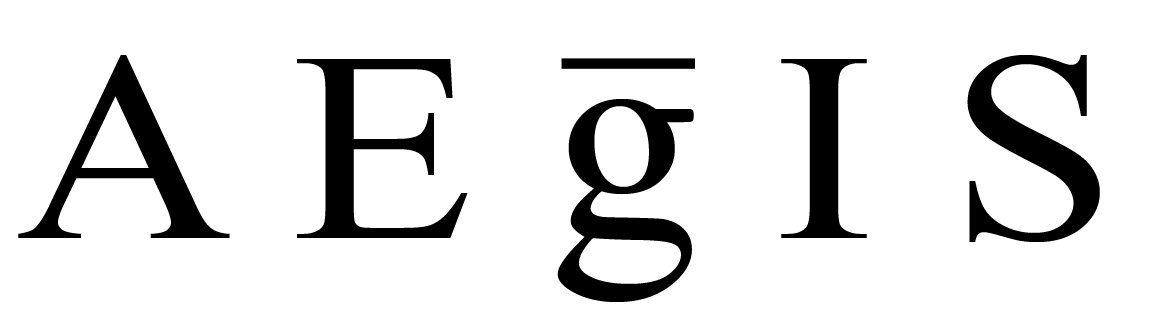
\includegraphics[scale=0.25]{aegisLogo.png} 
\caption{AEgIS's Logo}
\end{figure}

The weak equivalence principle, also known as universality of free fall, states that in the same field all bodies fall with the same acceleration, regardless of the mass and the composition. This principle has been thoroughly tested for the matter, but not for the antimatter: the most important goal of AEgIS experiment is to measure the weak equivalence principle for the anti-matter; to test this principle AEgIS measures gravitational interaction between matter (the earth) and anti-matter (anti-hydrogen). In the context of neutral antimatter, the gravitational interaction is of high interest, because it can potentially revealing new forces that violate the weak equivalence principle. Thomas Phillips, from Duke University, says: "If antimatter fell down faster, it would mean the discovery of at least one new force, probably two. If it fell up, it would mean our understanding of general relativity is incorrect". In a practical point of view AEgIS tries to mesure the time of flight and the vertical displacement of anti-hydrogen, by a moire deflectometer: this process is quite complex, and it is easier explain it by the following two images [TODO INSERT-THE-NUMBER-OF-THE-IMAGE].

\begin{figure}[H]
\centering
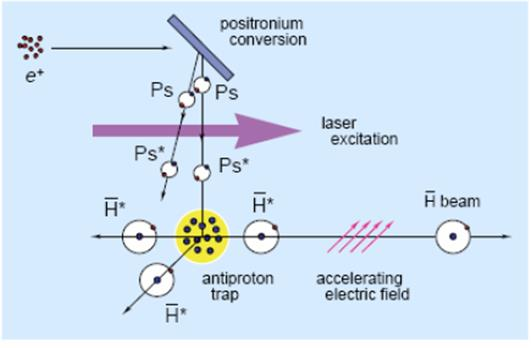
\includegraphics[scale=0.5]{AEgISScheme.png} 
\caption{AEgIS's Scheme, taken from "AEgIS experiment at CERN: measuring antihydrogen free-fall in Earth’s gravitational field to test WEP with antimatter" TODO INSERT-bibliographical-reference}
\end{figure}

In this first image we can see the process that allows to create some anti-hydrogen. To correctly explain this process it is better start with some definitions:


\begin{enumerate}

% 1
\item Positron: it is the correspondent of the electron in the anti-matter. It is an anti-electron, so an electron with positive electrical charge. It is indicated by "e+".

% 2
\item Positronium: it is an unstable system consisting of an electron and a positron, bound together into an exotic atom. It is indicated with "Ps".

% 3
\item Antiproton: it is the antiparticle of the proton. Antiprotons are stable, but they are typically short-lived since any collision with a proton will cause both particles to be annihilated in a burst of energy. It is indicated with $ \overline{p} $ (pronunced P-Bar).

\end{enumerate}


\begin{figure}[H]
\centering
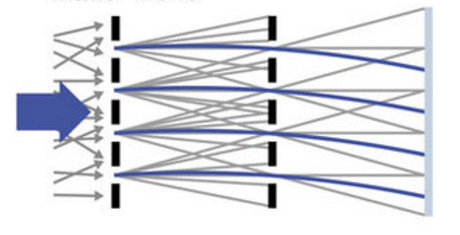
\includegraphics[scale=0.5]{MoireDeflectometer.png} 
\caption{Moiré Deflectometer's Scheme, taken from "AEgIS experiment at CERN: measuring antihydrogen free-fall in Earth’s gravitational field to test WEP with antimatter" TODO INSERT-bibliographical-reference}
\end{figure}


\section{User friendly Data analysis framework}

test todo point:

\begin{itemize}
\item 
a point todo todo todo
\end{itemize}
